\section{CFd\-Monitor  Class Reference}
\label{classCFdMonitor}\index{CFdMonitor@{CFd\-Monitor}}
{\tt \#include $<$CFd\-Monitor.h$>$}

Inheritance diagram for CFd\-Monitor::\begin{figure}[H]
\begin{center}
\leavevmode
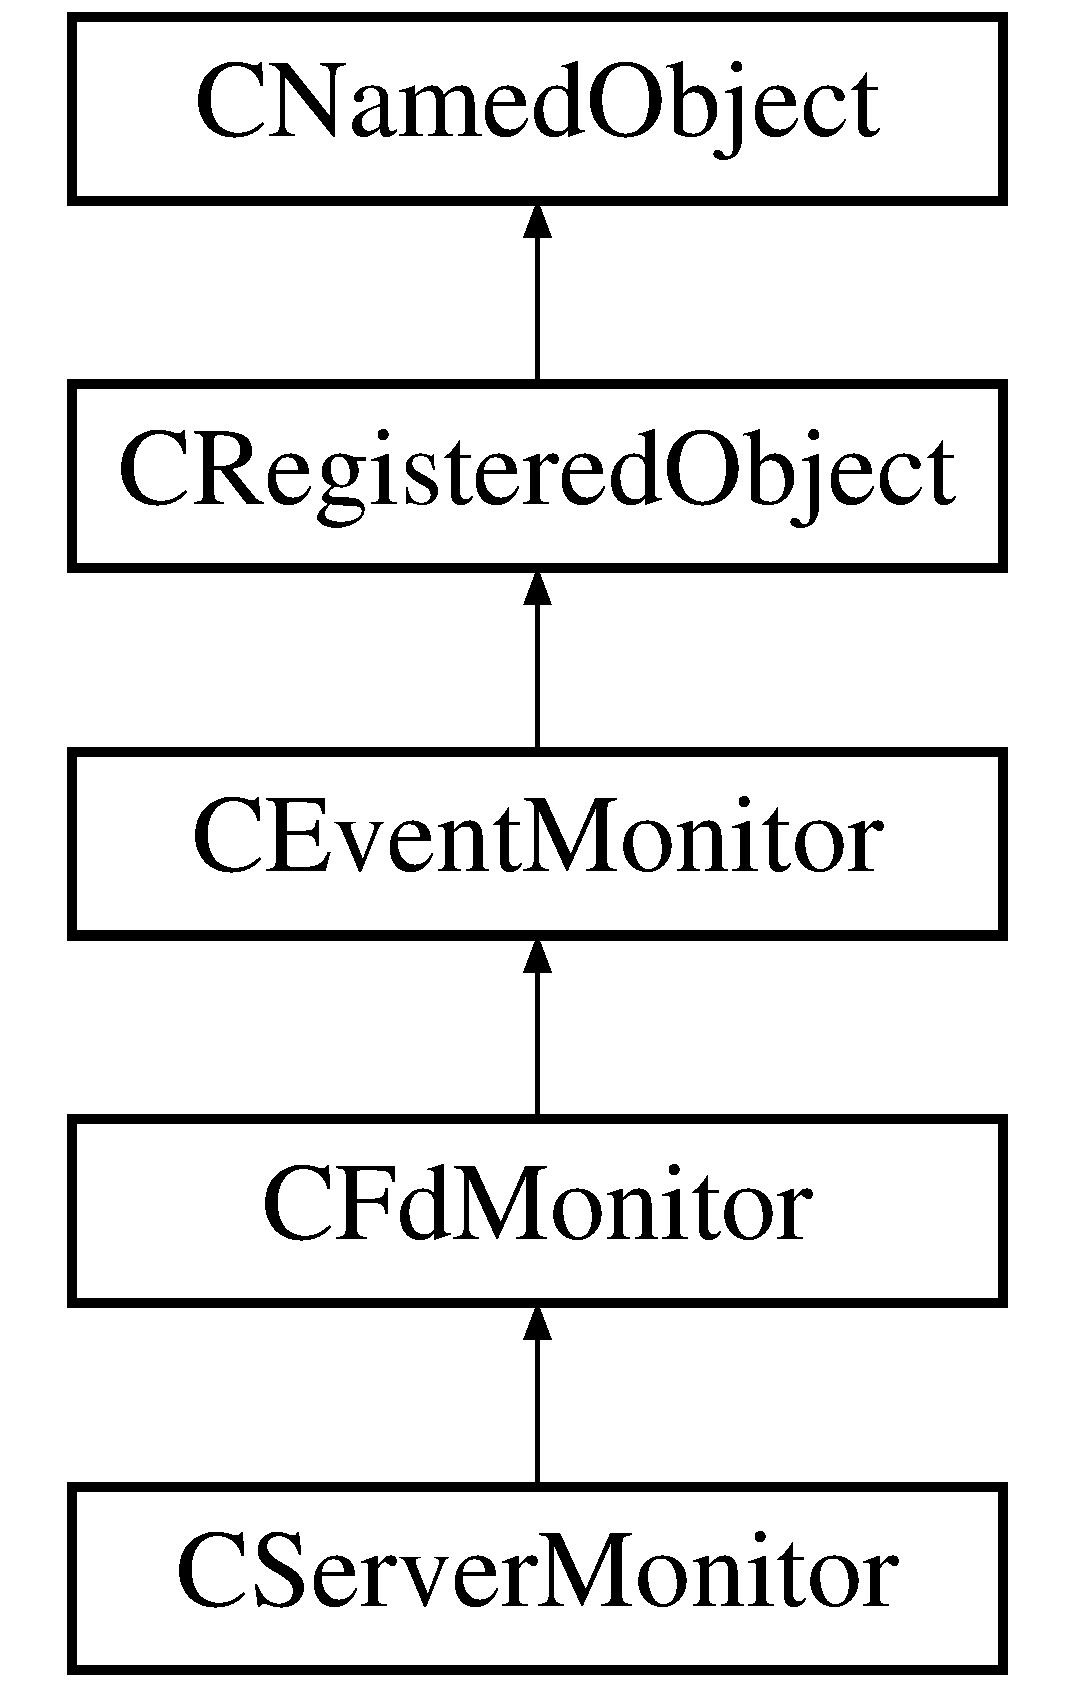
\includegraphics[height=5cm]{classCFdMonitor}
\end{center}
\end{figure}
\subsection*{Public Types}
\begin{CompactItemize}
\item 
enum {\bf Fd\-Conditions} \{ {\bf FD\_\-READABLE} = 0, 
{\bf FD\_\-WRITABLE} = 1, 
{\bf FD\_\-EXCEPTION} = 2
 \}
\end{CompactItemize}
\subsection*{Public Methods}
\begin{CompactItemize}
\item 
{\bf CFd\-Monitor} (int am\_\-n\-Fd, bool am\_\-f\-Timed\-Wait=true)
\item 
{\bf CFd\-Monitor} (const string \&r\-Name, int am\_\-n\-Fd, bool am\_\-f\-Timed\-Wait=true)
\item 
{\bf CFd\-Monitor} (const char $\ast$p\-Name, int am\_\-n\-Fd, bool am\_\-f\-Timed\-Wait=true)
\item 
int {\bf operator==} (const CFd\-Monitor \&a\-CFd\-Monitor) const
\item 
virtual {\bf $\sim$CFd\-Monitor} ()
\item 
int {\bf get\-Fd} () const
\item 
unsigned int {\bf get\-Condition\-Mask} () const
\item 
int {\bf get\-Last\-Event\-Mask} () const
\item 
void {\bf Monitor\-Readable} (bool f\-Readable=true)
\item 
void {\bf Monitor\-Writable} (bool f\-Writable=true)
\item 
void {\bf Monitor\-Exceptions} (bool f\-Exception=true)
\item 
virtual {\bf CEvent\-Monitor::result} {\bf operator()} ()
\item 
virtual string {\bf Describe\-Self} ()
\end{CompactItemize}
\subsection*{Protected Methods}
\begin{CompactItemize}
\item 
void {\bf set\-Fd} (const int am\_\-n\-Fd)
\item 
void {\bf set\-Condition\-Mask} (const unsigned int am\_\-n\-Condition\-Mask)
\item 
void {\bf set\-Last\-Event\-Mask} (const int am\_\-f\-Last\-Event\-Mask)
\end{CompactItemize}
\subsection*{Private Methods}
\begin{CompactItemize}
\item 
{\bf CFd\-Monitor} (const {\bf CRegistered\-Object} \&a\-CRegistered\-Object)
\item 
CFd\-Monitor {\bf operator=} (const {\bf CRegistered\-Object} \&a\-CRegistered\-Object)
\begin{CompactList}\small\item\em Assignment is forbidden for now.\item\end{CompactList}\end{CompactItemize}
\subsection*{Private Attributes}
\begin{CompactItemize}
\item 
int {\bf m\_\-n\-Fd}
\item 
unsigned int {\bf m\_\-n\-Condition\-Mask}
\item 
int {\bf m\_\-f\-Last\-Event\-Mask}
\end{CompactItemize}


\subsection{Detailed Description}
$\backslash$class: {\bf CFd\-Monitor.h}

This file defines the CFd\-Monitor class. Monitors activity on a file descriptor. A file descriptior can be  monitored for the logical or of any of the following conditions: Readable Writable Exception

Monitoring is done via the select(2) system service. Note that this can yield some unexpected results. For example, in some operating systems, tape drives are never considered readable without blocking.

Author: Jason Venema NSCL Michigan State University East Lansing, MI 48824-1321 mailto:{\tt venemaja@msu.edu} 



Definition at line 319 of file CFd\-Monitor.h.

\subsection{Member Enumeration Documentation}
\index{CFdMonitor@{CFd\-Monitor}!FdConditions@{FdConditions}}
\index{FdConditions@{FdConditions}!CFdMonitor@{CFd\-Monitor}}
\subsubsection{\setlength{\rightskip}{0pt plus 5cm}enum CFd\-Monitor::Fd\-Conditions}\label{classCFdMonitor_s3}


Mask of the last set of bits to be detected \begin{Desc}
\item[Enumeration values:]\par
\begin{description}
\index{FD_READABLE@{FD\_\-READABLE}!CFdMonitor@{CFd\-Monitor}}\index{CFdMonitor@{CFdMonitor}!FD_READABLE@{FD\_\-READABLE}}\item[{\em 
{\em FD\_\-READABLE}\label{classCFdMonitor_s3s0}
}]\index{FD_WRITABLE@{FD\_\-WRITABLE}!CFdMonitor@{CFd\-Monitor}}\index{CFdMonitor@{CFdMonitor}!FD_WRITABLE@{FD\_\-WRITABLE}}\item[{\em 
{\em FD\_\-WRITABLE}\label{classCFdMonitor_s3s1}
}]\index{FD_EXCEPTION@{FD\_\-EXCEPTION}!CFdMonitor@{CFd\-Monitor}}\index{CFdMonitor@{CFdMonitor}!FD_EXCEPTION@{FD\_\-EXCEPTION}}\item[{\em 
{\em FD\_\-EXCEPTION}\label{classCFdMonitor_s3s2}
}]\end{description}
\end{Desc}



Definition at line 329 of file CFd\-Monitor.h.

Referenced by CFd\-Reactor::On\-Event().

\subsection{Constructor \& Destructor Documentation}
\index{CFdMonitor@{CFd\-Monitor}!CFdMonitor@{CFdMonitor}}
\index{CFdMonitor@{CFdMonitor}!CFdMonitor@{CFd\-Monitor}}
\subsubsection{\setlength{\rightskip}{0pt plus 5cm}CFd\-Monitor::CFd\-Monitor (int {\em am\_\-n\-Fd}, bool {\em am\_\-f\-Timed\-Wait} = true)\hspace{0.3cm}{\tt  [inline]}}\label{classCFdMonitor_a0}




Definition at line 338 of file CFd\-Monitor.h.

References CNamed\-Object::Append\-Class\-Info(), m\_\-f\-Last\-Event\-Mask, m\_\-n\-Condition\-Mask, and m\_\-n\-Fd.\index{CFdMonitor@{CFd\-Monitor}!CFdMonitor@{CFdMonitor}}
\index{CFdMonitor@{CFdMonitor}!CFdMonitor@{CFd\-Monitor}}
\subsubsection{\setlength{\rightskip}{0pt plus 5cm}CFd\-Monitor::CFd\-Monitor (const string \& {\em r\-Name}, int {\em am\_\-n\-Fd}, bool {\em am\_\-f\-Timed\-Wait} = true)\hspace{0.3cm}{\tt  [inline]}}\label{classCFdMonitor_a1}




Definition at line 345 of file CFd\-Monitor.h.

References CNamed\-Object::Append\-Class\-Info(), m\_\-f\-Last\-Event\-Mask, m\_\-n\-Condition\-Mask, and m\_\-n\-Fd.\index{CFdMonitor@{CFd\-Monitor}!CFdMonitor@{CFdMonitor}}
\index{CFdMonitor@{CFdMonitor}!CFdMonitor@{CFd\-Monitor}}
\subsubsection{\setlength{\rightskip}{0pt plus 5cm}CFd\-Monitor::CFd\-Monitor (const char $\ast$ {\em p\-Name}, int {\em am\_\-n\-Fd}, bool {\em am\_\-f\-Timed\-Wait} = true)\hspace{0.3cm}{\tt  [inline]}}\label{classCFdMonitor_a2}




Definition at line 352 of file CFd\-Monitor.h.

References CNamed\-Object::Append\-Class\-Info(), m\_\-f\-Last\-Event\-Mask, m\_\-n\-Condition\-Mask, and m\_\-n\-Fd.\index{CFdMonitor@{CFd\-Monitor}!~CFdMonitor@{$\sim$CFdMonitor}}
\index{~CFdMonitor@{$\sim$CFdMonitor}!CFdMonitor@{CFd\-Monitor}}
\subsubsection{\setlength{\rightskip}{0pt plus 5cm}virtual CFd\-Monitor::$\sim$CFd\-Monitor ()\hspace{0.3cm}{\tt  [inline, virtual]}}\label{classCFdMonitor_a4}




Definition at line 369 of file CFd\-Monitor.h.\index{CFdMonitor@{CFd\-Monitor}!CFdMonitor@{CFdMonitor}}
\index{CFdMonitor@{CFdMonitor}!CFdMonitor@{CFd\-Monitor}}
\subsubsection{\setlength{\rightskip}{0pt plus 5cm}CFd\-Monitor::CFd\-Monitor (const {\bf CRegistered\-Object} \& {\em a\-CRegistered\-Object})\hspace{0.3cm}{\tt  [private]}}\label{classCFdMonitor_c0}




\subsection{Member Function Documentation}
\index{CFdMonitor@{CFd\-Monitor}!DescribeSelf@{DescribeSelf}}
\index{DescribeSelf@{DescribeSelf}!CFdMonitor@{CFd\-Monitor}}
\subsubsection{\setlength{\rightskip}{0pt plus 5cm}string CFd\-Monitor::Describe\-Self ()\hspace{0.3cm}{\tt  [virtual]}}\label{classCFdMonitor_a12}


Operation Type: Interface Implementation

Purpose: Uses the m\_\-s\-Class\-Path member to describe its class path, and returns a string containing this and its data member values. 

Reimplemented from {\bf CNamed\-Object} {\rm (p.\,\pageref{classCNamedObject_a8})}.

Reimplemented in {\bf CServer\-Monitor} {\rm (p.\,\pageref{classCServerMonitor_a8})}.

Definition at line 420 of file CFd\-Monitor.cpp.

References CNamed\-Object::Describe\-Self(), CEvent\-Monitor::get\-Timed\-Wait(), CEvent\-Monitor::get\-Timeout(), and m\_\-n\-Fd.

Referenced by main().\index{CFdMonitor@{CFd\-Monitor}!getConditionMask@{getConditionMask}}
\index{getConditionMask@{getConditionMask}!CFdMonitor@{CFd\-Monitor}}
\subsubsection{\setlength{\rightskip}{0pt plus 5cm}unsigned int CFd\-Monitor::get\-Condition\-Mask () const\hspace{0.3cm}{\tt  [inline]}}\label{classCFdMonitor_a6}




Definition at line 386 of file CFd\-Monitor.h.

References m\_\-n\-Condition\-Mask.

Referenced by main().\index{CFdMonitor@{CFd\-Monitor}!getFd@{getFd}}
\index{getFd@{getFd}!CFdMonitor@{CFd\-Monitor}}
\subsubsection{\setlength{\rightskip}{0pt plus 5cm}int CFd\-Monitor::get\-Fd () const\hspace{0.3cm}{\tt  [inline]}}\label{classCFdMonitor_a5}




Definition at line 381 of file CFd\-Monitor.h.

References m\_\-n\-Fd.

Referenced by CFd\-Reactor::On\-Event().\index{CFdMonitor@{CFd\-Monitor}!getLastEventMask@{getLastEventMask}}
\index{getLastEventMask@{getLastEventMask}!CFdMonitor@{CFd\-Monitor}}
\subsubsection{\setlength{\rightskip}{0pt plus 5cm}int CFd\-Monitor::get\-Last\-Event\-Mask () const\hspace{0.3cm}{\tt  [inline]}}\label{classCFdMonitor_a7}




Definition at line 391 of file CFd\-Monitor.h.

References m\_\-f\-Last\-Event\-Mask.

Referenced by CFd\-Reactor::On\-Event().\index{CFdMonitor@{CFd\-Monitor}!MonitorExceptions@{MonitorExceptions}}
\index{MonitorExceptions@{MonitorExceptions}!CFdMonitor@{CFd\-Monitor}}
\subsubsection{\setlength{\rightskip}{0pt plus 5cm}void CFd\-Monitor::Monitor\-Exceptions (bool {\em f\-Exception} = true)}\label{classCFdMonitor_a10}


Operation Type: Mutator

Purpose: Sets or clears the FD\_\-EXCEPTION bit in m\_\-n\-Condition\-Mask. 

Definition at line 344 of file CFd\-Monitor.cpp.

References FD\_\-EXCEPTION, and m\_\-n\-Condition\-Mask.

Referenced by main().\index{CFdMonitor@{CFd\-Monitor}!MonitorReadable@{MonitorReadable}}
\index{MonitorReadable@{MonitorReadable}!CFdMonitor@{CFd\-Monitor}}
\subsubsection{\setlength{\rightskip}{0pt plus 5cm}void CFd\-Monitor::Monitor\-Readable (bool {\em f\-Readable} = true)}\label{classCFdMonitor_a8}


Operation Type: Mutator

Purpose: Sets or clears the FD\_\-READABLE bit in m\_\-n\-Condition\-Mask. 

Definition at line 314 of file CFd\-Monitor.cpp.

References FD\_\-READABLE, and m\_\-n\-Condition\-Mask.

Referenced by main().\index{CFdMonitor@{CFd\-Monitor}!MonitorWritable@{MonitorWritable}}
\index{MonitorWritable@{MonitorWritable}!CFdMonitor@{CFd\-Monitor}}
\subsubsection{\setlength{\rightskip}{0pt plus 5cm}void CFd\-Monitor::Monitor\-Writable (bool {\em f\-Writable} = true)}\label{classCFdMonitor_a9}


Operation Type: Mutator

Purpose:  Sets or clears the FD\_\-WRITABLE bit in the m\_\-n\-Condition\-Mask attribute. 

Definition at line 329 of file CFd\-Monitor.cpp.

References FD\_\-WRITABLE, and m\_\-n\-Condition\-Mask.

Referenced by main().\index{CFdMonitor@{CFd\-Monitor}!operator()@{operator()}}
\index{operator()@{operator()}!CFdMonitor@{CFd\-Monitor}}
\subsubsection{\setlength{\rightskip}{0pt plus 5cm}{\bf CEvent\-Monitor::result} CFd\-Monitor::operator() ()\hspace{0.3cm}{\tt  [virtual]}}\label{classCFdMonitor_a11}


Operation Type: Interface Implementation

Purpose:

Implements a wait for a single file descriptor event as described in the mask. Returns one of: Occured - one of the masked conditions occured. Timed\-Out - Timeout was enabled and none of the conditions occured within the timeout. Error - An error condition ocurred. 

Implements {\bf CEvent\-Monitor} {\rm (p.\,\pageref{classCEventMonitor_a7})}.

Reimplemented in {\bf CServer\-Monitor} {\rm (p.\,\pageref{classCServerMonitor_a7})}.

Definition at line 367 of file CFd\-Monitor.cpp.

References CEvent\-Monitor::Error, FD\_\-EXCEPTION, FD\_\-READABLE, FD\_\-WRITABLE, CEvent\-Monitor::get\-Timed\-Wait(), CEvent\-Monitor::get\-Timeout(), m\_\-f\-Last\-Event\-Mask, m\_\-n\-Condition\-Mask, m\_\-n\-Fd, CEvent\-Monitor::Occurred, and CEvent\-Monitor::Timed\-Out.\index{CFdMonitor@{CFd\-Monitor}!operator=@{operator=}}
\index{operator=@{operator=}!CFdMonitor@{CFd\-Monitor}}
\subsubsection{\setlength{\rightskip}{0pt plus 5cm}CFd\-Monitor CFd\-Monitor::operator= (const {\bf CRegistered\-Object} \& {\em a\-CRegistered\-Object})\hspace{0.3cm}{\tt  [private]}}\label{classCFdMonitor_c1}


Assignment is forbidden for now.



Reimplemented from {\bf CEvent\-Monitor} {\rm (p.\,\pageref{classCEventMonitor_c1})}.

Referenced by CServer\-Monitor::operator=().\index{CFdMonitor@{CFd\-Monitor}!operator==@{operator==}}
\index{operator==@{operator==}!CFdMonitor@{CFd\-Monitor}}
\subsubsection{\setlength{\rightskip}{0pt plus 5cm}int CFd\-Monitor::operator== (const CFd\-Monitor \& {\em a\-CFd\-Monitor}) const\hspace{0.3cm}{\tt  [inline]}}\label{classCFdMonitor_a3}




Definition at line 360 of file CFd\-Monitor.h.

References m\_\-f\-Last\-Event\-Mask, m\_\-n\-Condition\-Mask, m\_\-n\-Fd, and CEvent\-Monitor::operator==().

Referenced by CServer\-Monitor::operator==().\index{CFdMonitor@{CFd\-Monitor}!setConditionMask@{setConditionMask}}
\index{setConditionMask@{setConditionMask}!CFdMonitor@{CFd\-Monitor}}
\subsubsection{\setlength{\rightskip}{0pt plus 5cm}void CFd\-Monitor::set\-Condition\-Mask (const unsigned int {\em am\_\-n\-Condition\-Mask})\hspace{0.3cm}{\tt  [inline, protected]}}\label{classCFdMonitor_b1}




Definition at line 404 of file CFd\-Monitor.h.

References m\_\-n\-Condition\-Mask.\index{CFdMonitor@{CFd\-Monitor}!setFd@{setFd}}
\index{setFd@{setFd}!CFdMonitor@{CFd\-Monitor}}
\subsubsection{\setlength{\rightskip}{0pt plus 5cm}void CFd\-Monitor::set\-Fd (const int {\em am\_\-n\-Fd})\hspace{0.3cm}{\tt  [inline, protected]}}\label{classCFdMonitor_b0}




Definition at line 399 of file CFd\-Monitor.h.

References m\_\-n\-Fd.\index{CFdMonitor@{CFd\-Monitor}!setLastEventMask@{setLastEventMask}}
\index{setLastEventMask@{setLastEventMask}!CFdMonitor@{CFd\-Monitor}}
\subsubsection{\setlength{\rightskip}{0pt plus 5cm}void CFd\-Monitor::set\-Last\-Event\-Mask (const int {\em am\_\-f\-Last\-Event\-Mask})\hspace{0.3cm}{\tt  [inline, protected]}}\label{classCFdMonitor_b2}




Definition at line 409 of file CFd\-Monitor.h.

References m\_\-f\-Last\-Event\-Mask.

\subsection{Member Data Documentation}
\index{CFdMonitor@{CFd\-Monitor}!m_fLastEventMask@{m\_\-fLastEventMask}}
\index{m_fLastEventMask@{m\_\-fLastEventMask}!CFdMonitor@{CFd\-Monitor}}
\subsubsection{\setlength{\rightskip}{0pt plus 5cm}int CFd\-Monitor::m\_\-f\-Last\-Event\-Mask\hspace{0.3cm}{\tt  [private]}}\label{classCFdMonitor_o2}


Conditions which will be monitored by  the monitor for the file descriptor. 

Definition at line 324 of file CFd\-Monitor.h.

Referenced by CFd\-Monitor(), get\-Last\-Event\-Mask(), operator()(), operator==(), and set\-Last\-Event\-Mask().\index{CFdMonitor@{CFd\-Monitor}!m_nConditionMask@{m\_\-nConditionMask}}
\index{m_nConditionMask@{m\_\-nConditionMask}!CFdMonitor@{CFd\-Monitor}}
\subsubsection{\setlength{\rightskip}{0pt plus 5cm}unsigned int CFd\-Monitor::m\_\-n\-Condition\-Mask\hspace{0.3cm}{\tt  [private]}}\label{classCFdMonitor_o1}


File descriptor which will be monitored by the monitor 

Definition at line 322 of file CFd\-Monitor.h.

Referenced by CFd\-Monitor(), get\-Condition\-Mask(), Monitor\-Exceptions(), Monitor\-Readable(), Monitor\-Writable(), operator()(), operator==(), and set\-Condition\-Mask().\index{CFdMonitor@{CFd\-Monitor}!m_nFd@{m\_\-nFd}}
\index{m_nFd@{m\_\-nFd}!CFdMonitor@{CFd\-Monitor}}
\subsubsection{\setlength{\rightskip}{0pt plus 5cm}int CFd\-Monitor::m\_\-n\-Fd\hspace{0.3cm}{\tt  [private]}}\label{classCFdMonitor_o0}




Definition at line 321 of file CFd\-Monitor.h.

Referenced by CFd\-Monitor(), Describe\-Self(), get\-Fd(), operator()(), operator==(), and set\-Fd().

The documentation for this class was generated from the following files:\begin{CompactItemize}
\item 
{\bf CFd\-Monitor.h}\item 
{\bf CFd\-Monitor.cpp}\end{CompactItemize}
